\chapter{Sistemas de generación de mosaico}
\label{capitulo2}
\lhead{Capítulo 2. \emph{Sistemas de generación de mosaico}}

En este capítulo se presenta una revisión teórica del estado actual de las investigaciones que se han desarrollado en el área de procesamiento de imágenes, aplicado a la construcción de mosaicos, además de una reseña histórica de la evolución de dichos métodos. Debido a que la construcción de mosaicos ha sido y sigue siendo un área de investigación muy activa, existe una gran variedad de métodos y técnicas que se han empleado para este fin. Con el objetivo de recopilar esta información de manera estructurada, se presenta una clasificación de estos algoritmo en base al modo de abordar los módulos principales para la elaboración de estos mapas.

Con esto se pretende recuperar y trascender el conocimiento acumulado en esta área de estudio, además de familiarizar al lector con los conceptos básicos, necesarios para la comprensión del presente trabajo. Seguidamente se presenta el modelo del sistema de generación de mosaico propuesto en base a los algoritmos y técnicas que se han utilizado en las investigaciones mas recientes. Finalmente se introduce la librería de procesamiento de imágenes que se seleccionó para la implementación de todos los módulos necesarios.

\section{Estado del arte}

La elaboración de mosaicos para la construcción de mapas del suelo, se ha desarrollado incluso antes desde la era digital de la computadoras. Desde que el proceso de registrar fotografías ha existido, se comenzaron a usar para elaborar mapas topográficos \cite{primeros-mapas}, donde imágenes adquiridas a partir de globos aerostáticos o altas colinas eran unidas manualmente. Posteriormente, producto de los avances en materia de aeronáutica, el interés por la aerofotografía se incrementó en gran medida. En este mismo sentido se utilizaban aviones para el registro de imágenes a mayores altitudes, logrando cubrir mayores áreas en menor cantidad de tiempo. Pero debido a que no se alcanzaba suficiente altura, y se mantenía la necesidad de registrar grandes áreas, era requerido que los mapas se construyan mediante fotografías que se superpongan, de igual forma esta tarea se llevaba a cabo mediante técnicas manuales por medio de expertos.

La necesidad de registrar áreas aun mas grandes siguió avanzando, motivado por la llegada de los satélites que eran capaces de enviar a tierra la información que obtenían de las cámaras. Los avances tecnológicos en materia de computación, y el creciente aumento de datos para esta aplicación, promovieron el desarrollo de técnicas de procesamiento digital de imágenes para dar solución a este tipo de problemas.

Con el desarrollo de cámaras cada vez mas pequeñas y portátiles, así como también la llegada de vehículos no tripulados mas compactos ---ROV, UAV, AUV---, se produjeron grandes avances y nuevas técnicas por parte de centros de investigación en el área de la física, robótica y visión por computadora, que buscaron aportar soluciones para la realización automática de mosaicos. Esta vez, con un creciente enfoque en las aplicaciones mas desafiantes como los ambientes submarinos.

Para explicar el proceso en el que consiste construir un mapa del suelo a partir de fotografías, lo podemos separar en tres simples pasos. Si bien, éste se ilustran gráficamente en la figura \ref{imagen:mosaic-process}, a continuación se explica cada una de estas etapas.

\begin{itemize}
	\item \textbf{Registro:} De su termino en inglés \textit{image-registration}, consiste en establecer la correspondencia geomántica entre las imágenes que componen la misma escena. Para esto, es necesario estimar la transformación geométrica que logra alinear dichas imágenes en un mismo plano.
	
	\item \textbf{Alineación:} También llamada proyección, consiste en alinear las imágenes registradas en un sistema de referencia común, es decir, con respecto a un plano re referencia. En este caso se utiliza la transformación geométrica calculada en el paso anterior.
	
	\item \textbf{Fusión:} En este paso se busca corregir los errores fotométricos o discontinuidades, presentes en el mosaico luego del proceso de alineación. Estos errores aparecen, producto de errores en la estimación de las transformaciones o a cambios en la perspectiva de los objetos observados.
\end{itemize}

Si bien, se han propuesto una gran cantidad de algoritmos por parte de distintos grupos de investigación en todo el mundo, esta tarea aun sigue siendo desafiante, debido mayormente a los procesos de registro y fusión de las imágenes.

\begin{figure}[H]
	\centerline{
		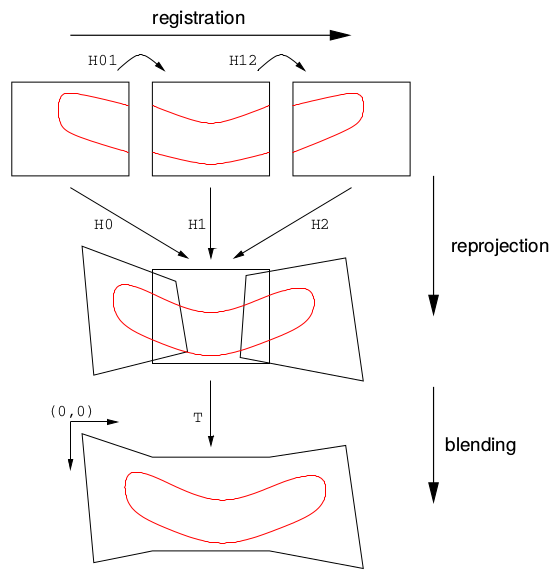
\includegraphics[width=10cm]{registration-process}}
	\caption[Proceso básico para la generación de mosaico]{Proceso básico para la generación de mosaico, adaptado de \cite{capel}}
	\label{imagen:mosaic-process}
\end{figure}

Específicamente la etapa para estimar correspondencias entre las imágenes es un problema complicado, en principio debido a la naturaleza no plana de los suelos estudiados; por otro lado la reducción de discontinuidades, o inconsistencias entre imágenes consecutivas sigue siendo una tarea desafiante, en este caso debido a fuertes cambios de exposición o errores en la etapa de registro. Es por esto que la mayoría de avances e implementaciones en esta área, están encaminados en resolver estos dos problemas principales, o bien mejorar los resultados de trabajos previos.

De esta forma se propone una clasificación de los algoritmos de mosaicos, basada en como estos abordan los procesos de registro y fusión. Además, para cada clasificación se realiza una breve revisión teórica de cada categoría, así como también los diferentes métodos y modificaciones que han aplicado diversos desarrolladores. en la figura \ref{imagen:clasificacion} se puede apreciar esta clasificación.

\begin{figure}[H]
	\centerline{
		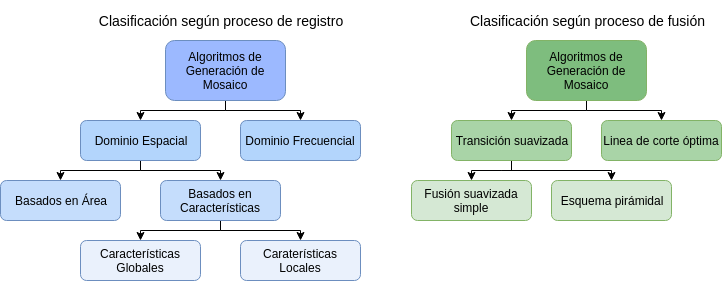
\includegraphics[width=15cm]{clasificacion}}
	\caption[Clasificación de los algoritmos de generación de mosaico]{Clasificación de los algoritmos de generación de mosaico según como aborden las etapas de registro y fusión}
	
	\label{imagen:clasificacion}
\end{figure}


\section*{Clasificación basada en el registro de imágenes}

Este proceso es muy importante para la creación de mosaicos, y básicamente es la base para estos. Cuando se registran imágenes, primero lo que se busca es encontrar la relación, o la correspondencia entre estas, teniendo en cuanta que pudieron haber sido capturadas desde distintos puntos de vista, distintos instantes de tiempo, distinta perspectiva, o incluso distintas cámaras. Luego de encontrar las zonas o puntos correspondientes, se busca estimar una matriz de transformación geométrica que permita alinearlas todas en un sistema de referencia común. Se puede decir que el registro ha sido exitoso, si se logra estimar una matriz de transformación tal que todos los puntos correspondientes se puedan unir.

Las relaciones entre las imágenes se pueden establecer utilizando distintos métodos, ya sea, emparejando puntos coincidentes, regiones enteras, o bien usando la propiedad de correlación de fase en el dominio de la frecuencia. Si bien se cuenta con algoritmos de generación de mosaico que realizan el registro de imágenes basados en datos de navegación, como el GPS (del inglés: Global Positioning System), o instrumentos de medición inercial IMU (del inglés: Inertial Measurement Unit), para estimar el movimiento de los vehículos y así establecer una relación entre las imágenes basado en el movimiento de la cámara, en este trabajo solo se discutirán técnicas que utilicen únicamente una cámara monocular como sensor de entrada. Dicho esto, estos métodos para establecer correspondencias son discutidos a continuación.

\subsection*{Algoritmos en el dominio espacial}

Los algoritmos en esta categoría utilizan la información de los píxeles para establecer la relación entre imágenes, es decir, se utiliza el valor de los píxeles (intensidad) y se trata de establecer la correspondencia de estos según la ubicación en la que se encuentran. Estos se pueden separar en dos técnicas principales: basados en área o en características.

% Basados en Area

Los algoritmos basados en área, buscan relacionar dos ventanas o regiones en dos imágenes que correspondan a la misma escena. El concepto principal consiste en mover la región de interés desde la primera imagen hacia la segunda, buscando que la diferencia entre las intensidades sea la menor posible, es decir,  se trata de estimar la mejor matriz de transformación que logre reducir la diferencia de intensidades al alinear las regiones estudiadas \cite{nccvsmi}. Algunos trabajos importantes en esta clasificación utilizaron algoritmos como NCC (siglas del inglés: Normalized Cross Correlation) \cite{ncc}, y el MI (siglas del inglés: Mutual Information) \cite{mi}, donde estos proporcionan una métrica de igualdad entre dos imágenes.

El el primer caso, el NCC mide la similitud entre las regiones estudiadas según los valores de intensidades, mientras que el MI la mide en base a la cantidad de información que comparten estas imágenes en términos de entropía. Al emplear esta técnica se logra emparejar las imágenes a nivel de píxel. Si bien se logran buenos resultados, este tipo de algoritmo requiere un alto nivel de superposición entre las imágenes de entrada. Además, el proceso de iterar para optimizar los parámetros de transformación y el calculo del error para cada píxel sobre las regiones, se convierte computacionalmente costoso.


% Basados en Características

Para reducir el tiempo de computo, se utilizan algoritmos basados en la relación de características, en los cuales se tratan de detectar puntos o regiones en distintas imágenes, que correspondan con la misma ubicación. Estas características detectadas se pueden evidenciar en forma de puntos aislados, curvas continuas o regiones conectadas. Luego se puede encontrar la transformación geométrica que relaciona las características de origen con las de destino, en muchos casos resolviendo un sistema de ecuaciones. En este caso, el proceso de registro así como también el resultado del mosaico, será tan bueno como el algoritmo de detección que se utilice.

Tal y como se mencionaron los tipos de características que se pueden extraer, podemos clasificar de forma general los algoritmos de detección. Ya sea si trabajan con características locales, como lo son aquello que detectan puntos aislados. o mas globales como los basados en detección de contornos.

\subsubsection*{Detectores locales}

Al usar este tipo de algoritmos se busca encontrar la relación entre una serie de puntos dispersos que se corresponden entre dos imágenes, donde las características locales mas comunes que se suelen detectar serian esquinas, bordes, manchas, entre otros. Posteriormente el proceso de registro se completa al estimar la transformación geométrica con dicha relación de puntos, en este caso resolviendo un sistema de ecuaciones.

Una de las ventajas principales de esta técnica para la generación de mosaicos, es que puede trabajar con imágenes consecutivas que no posean un alto nivel de cobertura. Siempre y cuando la cantidad de puntos detectados, y correctamente emparejados entre el par de imágenes supere el mínimo necesario para la solución del sistema de ecuaciones.

Diversos algoritmos detectores de características locales se han venido desarrollando desde hace mucho tiempo \cite{harris,sift,surf,fast,brief,orb,kaze,akaze}, y en la actualidad estos avances han permitido que el uso de este método traiga consigo muchas ventajas sobre el resto, desde variedad de aplicaciones, robustez ante distinto tipo de escenas, y velocidad de computo (siempre en función del detector a utilizar), lo que lo convierte en uno de los mas usados para la construcción de mosaicos.

\subsubsection*{Detectores globales}

Al utilizar este tipo de detectores, se busca encontrar formas, contornos, texturas, o regiones sobresalientes que se mantengan invariantes ante cambios del punto de vista o iluminación \cite{high-level}. Al igual que con los detectores locales, aquí se busca extraer tanto la posición, como el tamaño y la orientación de estas regiones.

El resto del proceso para completar la etapa de registro se mantiene igual con este método, donde la transformación geométrica se obtiene a partir de la correspondencia entre las posiciones y orientaciones de las regiones de interés que se lograron extraer. Si bien tienen buen rendimiento ante cambios de movimiento desafiantes, su uso implica un aumento en el tiempo de computo.

\subsection*{Algoritmos en el dominio frecuencial}

Ya se ha visto que los algoritmos que operan en el dominio espacial cubren la mayoría de las aplicaciones e investigaciones. Sin embargo se pueden encontrar métodos que obtienen los parámetros óptimos para la transformación a partir de cálculos en el dominio de la frecuencia. 

Estos algoritmos utilizan la propiedad de correlación de fase para lograr su objetivo. Teniendo un par de imágenes que se encuentran relacionadas por una simple traslación, el funcionamiento consiste en calcular la correspondiente transformada de \textit{Fourier}, luego el espectro de la potencia cruzada entre ambas. De aquí, se asegura que la fase del espectro de la potencia cruzada corresponde con la diferencia de traslación entre las dos imágenes. Finalmente el proceso continua similarmente a los métodos anteriores, alineando las imágenes según la transformación obtenida, seguido del proceso de fusionarlas.

Tal y como se explicó este proceso para una traslación, se tienen diversos trabajos como \cite{phase-rot} que añaden modificaciones para permitir otro tipo de transformaciones como la rotación, e incluso otros que admiten cambios en la escala \cite{phase-scale}. Si bien, los trabajos mencionados presentaron importantes, se requiere de un buen porcentaje de cobertura entre las imágenes, y además presentan limitaciones en los grados de libertad de las transformaciones geométricas que se pueden estimar.


\section*{Clasificación basada en la fusión de imágenes}

Si bien el proceso de registro de imágenes es fundamental para lograr un mosaico correcto, el paso final de unir las imágenes también es de gran importancia. Teniendo en cuenta que se busca aparentar que todas las imágenes componen una sola, es vital que se logre un mapa final sin inconsistencias o discontinuidades producto de los cambios en iluminación, objetos en movimiento, entre otros.

Debido a la importancia de este paso, numerosos métodos para lidiar con este tipo de problemas se han desarrollado, lo que nos permite también clasificar los algoritmos de generación de mosaico según como aborden este problema. Entre los métodos mas utilizados encontramos: fusionar las imágenes mediante cambios suavizados o búsqueda de la mejor linea de corte.

\subsection*{Transición suavizada}

Los algoritmos de esta categoría tratan de minimizar la diferencia entre dos imágenes, buscando que el cambio entre los bordes de estas sea imperceptible. El método mas simple para fusionar dos imágenes bajo esta técnica, consiste en realizar una suma ponderada sobre el área de superposición entre ambas, ponderando la intensidad de cada imagen a la mitad. Al realizar esta operación se suelen tener efectos indeseados como el efecto fantasma, en el cual se pueden observar duplicados del mismo objeto con cierto nivel de desvanecimiento. Esto de sebe a errores en el proceso de alineación de las imágenes, diferencia en la iluminación, o incluso a objetos móviles. 

Para evitar esto, se utiliza un proceso de fusión que consiste en realizar una suma ponderada entre ambas imágenes, pero dando mayor peso a las regiones que se encuentren mas cerca del centro de la imagen, y menor a aquellas que se encuentren cerca el borde. Si bien, se logra reducir posibles discontinuidades entre los bordes originales, el efecto fantasma aun se puede apreciar para imágenes con fuertes problemas de alineación.

Considerando este problema, y con el objetivo de realizar una unión mas robusta, se desarrolló un esquema piramidal de fusión ponderada. El proceso consiste en obtener una imagen laplaciana para distintos tamaños de escala, formando así una pirámide, al mismo tiempo se va creando para cada nivel de la pirámide una mascara difuminada por el efecto del filtro gaussiano de dicha escala. Luego para cada nivel de la pirámide se aplica el algoritmo de fusión ponderada descrito previamente donde la mascara  difuminada pondera el valor de cada píxel. Entre los trabajos que aplican este algoritmo obteniendo resultados notables se tiene \cite{multiband}, logrando reducir en gran medida el efecto duplicado en las regiones de superposición.

\subsection*{Linea de corte óptima}

En lugar de buscar reducir las posibles discontinuidades a partir de una suave transición a través del borde entre dos imágenes, tal y como lo hacen los algoritmo previos, en este tipo de algoritmos se busca modificar este borde. Es decir, se trata de encontrar la linea de corte en el área de superposición que logre reducir la discontinuidad de texturas entre ambas imágenes. La diferencia principal de este método sobre los anteriores, es que se toma en cuenta la información presente en la región que se desea fusionar, permitiendo que se logre remover errores producidos por el efecto paralaje, o debido a objetos móviles dentro de la escena. Por otra parte, como las regiones resultantes luego de la linea de corte no se comparten información, se pueden presentar discontinuidades producto de grandes diferencias de iluminación.

En esta sección podemos destacar el trabajo en \cite{zhang}, que presenta resultados robustos ante imágenes con alto efecto paralaje. En este se busca el área para el cual ambas imágenes presentan mejor similitud ---llamada área de costura-local---, y se busca una linea de corte que bordee esta región. Por otro lado tenemos trabajos como el presentado en \cite{watershed}, donde se busca la linea de corte que minimiza la diferencia entre los gradientes en el área de superposición, a través de un modelado por grafos, y resolviendo el algoritmo flujo-máximo/mínimo-corte \cite{maxflow} para encontrar la línea deseada.


\section{Esquema propuesto}

En base a los métodos estudiados en la sección anterior, se plantea el siguiente esquema para la construcción automática de mosaicos:

En primer lugar, se propone utilizar un esquema basado en características para la etapa de registro de imágenes, específicamente, utilizar algoritmos detectores de características locales. El uso de esta técnica permite que se pueda trabajar con imágenes consecutivas que no tengan un elevado nivel de superposición. Además, la gran variedad de algoritmos presentes de esta categoría permite trabajar bajo un gran número de ambientes, presentando robustez ante variados tipos de condiciones. 

Por otro lado, evaluando visualmente los resultados obtenidos en las distintas técnicas de fusión, se pretende implementar una combinación en los algoritmos que fueron mas eficientes bajo condiciones de alto efecto paralaje, presencia de objetos móviles, cambios en la iluminación, entre otros. En este caso, se buscaría la linea de corte óptima y luego se aplica una fusión bajo un esquema piramidal.

Si bien el registro y la fusión constituyen las etapas mas importantes, diversos métodos para lograr corregir errores de distorsión y proyección se han desarrollado de la mano de muchos grupos de investigación. Evaluando entre los presentes, se plantea implementar el modelo de sub mosaicos propuesto por \textit{F. Bellavia et. al.} en \cite{bellavia-ransac,bellavia-ref}, el cual se presentará detalladamente en el siguiente capítulo. Explicado brevemente, estos algoritmos buscan reducir errores provenientes de la sección de registro, y toman en consideración algunos aspectos importantes que logran reducir distorsiones geométricas en el mosaico final. 

Finalmente, tomando en cuenta algunas observaciones y recomendaciones de los trabajos consultados, se propone implementar un módulo de corrección de color con el objetivo de reducir las diferencias de intensidades entre los bordes de las imágenes consecutivas. Adicionalmente en el esquema se agregan algunas técnicas propuestas en \cite{grid} para añadir robustez al sistema propuesto. El esquema propuesto se puede observar en la figura \ref{imagen:esquema}, donde cada uno de estos módulos serán explicados en detalle en los capítulos siguientes.

\begin{figure}[H]
	\centerline{
		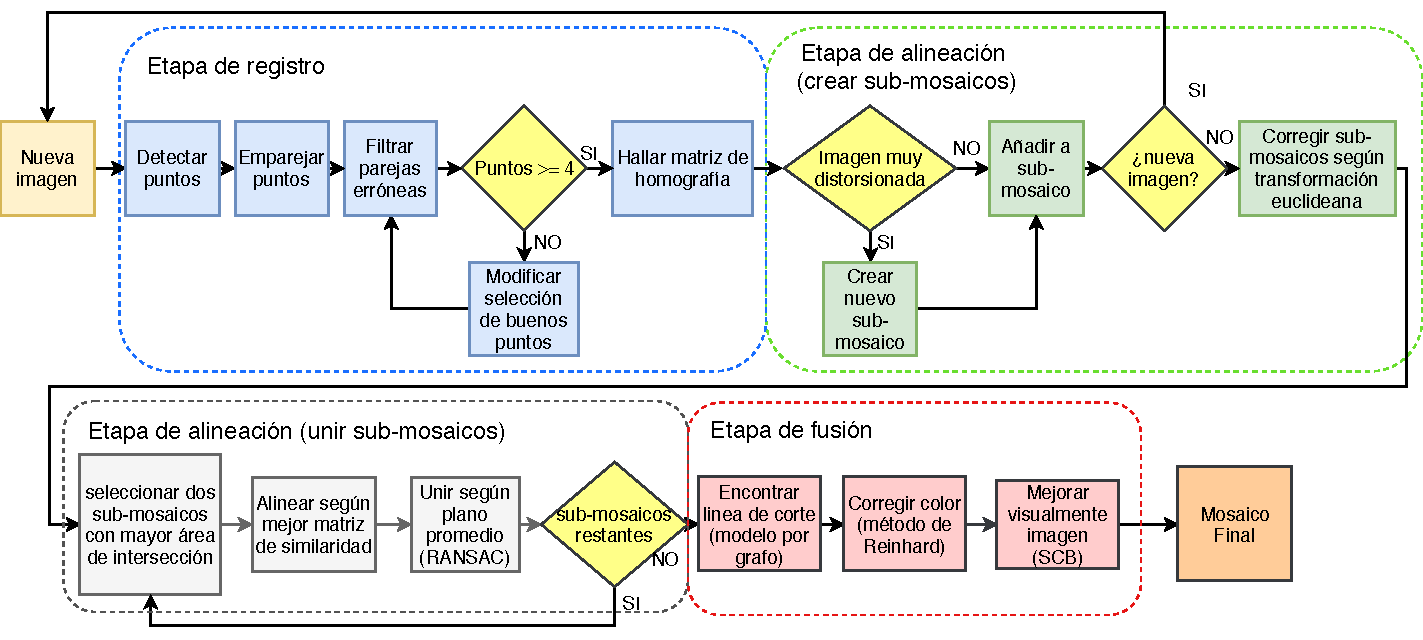
\includegraphics[width=1.21\textwidth]{esquema-general}}
		\caption{Esquema propuesto para la construcción del mosaico}
	\label{imagen:esquema}
\end{figure}

\section{Librería de desarrollo}

\subsection{OpenCV}

\begin{wrapfigure}{R}{5cm}
	\begin{center}
		\vspace*{-0.2in}
		
\includegraphics[width=4cm]{opencv}
	\end{center}
	\caption{Logo de la librería OpenCV}
\end{wrapfigure}

Para la implementación de los módulos previamente descritos, es necesario el uso de librerías y entornos de trabajo, que permitan un manejo eficiente de las imágenes. Además, el uso de de plataformas que se encuentren estandarizadas en esta área de estudio, facilita que el desarrollo del presente trabajo siga avanzando de la mano de futuros desarrolladores. En base a esto, se seleccionó la librería OpenCV\footnote{\url{http://opencv.org/}} para la implementación de los módulos necesarios en el sistema de generación de mosaico.

OpenCV (del inglés: \textit{Open Source Computer Vision}) es una librería de procesamiento de imágenes desarrollada por la empresa Intel\footnote{\url{http://www.intel.com}} en el año 1999. Esta librería ofrece un gran numero de algoritmos optimizados (actualmente mas de 2.500), el cual proporciona un entorno de desarrollo altamente eficiente para aplicaciones de procesamiento de imágenes. Asimismo presenta una gran aceptación por parte de los usuarios en el mundo académico y comercial, con mas de 47 mil usuarios activos, y un numero de descargas que supera los 14 millones.

Esta plataforma tiene soporte para distintos sitemas operativos, como \textit{Windows, Linux, Mac OS, iOS y Android.} Ademas de tener la posibilidad de trabajarla con diversos lenguajes de programación como: C++, Python, JavaScript. La motivación de el presente trabajo se encuentra orientada al desarrollo de una aplicación que en un futuro pueda ser embebida en un sistema de navegación automático, con lo cual el soporte de un lenguaje de bajo nivel como C++, puede permitir el desarrollo de un algoritmo con suficiente velocidad de computo para este fin.

Por otra parte, esta librería presenta soporte para trabajar con la arquitectura de de cálculo paralelo \textit{CUDA} (del inglés: \textit{Compute Unified Device Architecture}) de la empresa NVIDIA\footnote{\url{http://www.nvidia.com}}, con la cual se puede aprovechar el uso de las unidades de procesamiento gráfico para acelerar el rendimiento del algoritmo que se implemente. Cabe destacar que los equipos presentes en el laboratorio del \textit{GIDM} tienen disponible tarjetas gráficas con este soporte.

